% Quantization and ASR Noise in On-Device Voice Agents: Independent, Not Compounding
% Self-contained arXiv-ready preprint. Compiles with pdflatex alone (no external
% .sty). To retarget to a workshop: swap \documentclass for the venue style
% (e.g. neurips_2024 for ENLSP, or the ACL style for SustaiNLP) and move the
% thebibliography into a .bib if the template expects one.
\documentclass[11pt]{article}
\usepackage[margin=1in]{geometry}
\usepackage[T1]{fontenc}
\usepackage{lmodern}
\usepackage{microtype}
\usepackage{booktabs}
\usepackage{graphicx}
\usepackage{amsmath}
\usepackage{amssymb}
\usepackage{xcolor}
\usepackage[round]{natbib}
\usepackage[hidelinks]{hyperref}

\graphicspath{{results/}}
\newcommand{\code}[1]{\texttt{#1}}

\title{\bfseries Quantization and ASR Noise in On-Device\\
Voice Agents: Independent, Not Compounding}
\author{Sakthivinash Balu\\
\small Independent Researcher \quad\texttt{sakthivinashb@gmail.com} \quad ORCID: \href{https://orcid.org/0009-0009-4091-9795}{0009-0009-4091-9795}\\
\small Code \& data: \url{https://github.com/SAKTHIVINASH2/quant-asr-voice-agents}}
\date{Preprint --- November 2026}

\begin{document}
\maketitle

\begin{abstract}
On-device voice assistants increasingly pair a small quantized LLM with streaming
ASR and TTS, yet two deployment fears remain untested \emph{together}: that
aggressive quantization cripples the agent, and that quantization and noisy ASR
input compound into a quality cliff. We measure both inside a CPU
ASR$\rightarrow$LLM$\rightarrow$TTS pipeline. First, the LLM stage dominates
end-to-end latency (76--84\%), no quantization level meets a one-second
conversational budget, and quantization is not a reliable latency lever on CPU ---
decode speed varies non-monotonically with bit-width and is swamped by thermal/load
state. Second, on tool-calling (BFCL, $n{=}400$, two model families), there is
\textbf{no quantization$\times$noise interaction}: ASR noise roughly halves argument
slot-filling accuracy \emph{uniformly} across bit-widths, and a conservative 95\% CI
excludes any interaction larger than ${\sim}0.1$ exact-match. This null holds under
both a synthetic and a phonetically-grounded noise model, on both families. The
\emph{standalone} cost of 2-bit quantization on clean input is model-dependent
(negligible for Qwen2.5-3B, ${\sim}15$ exact-match points for Llama-3.2-3B), but ASR
noise never compounds it; function selection and JSON-format fidelity stay robust
throughout. The failure modes are thus independent: quantization can be chosen on its
clean-input merits without fear of a noise-amplified cliff, while the binding
constraints are latency and ASR quality. We release a reproducible evaluation harness
for on-device voice agents.
\end{abstract}

\noindent\textbf{Keywords:} on-device LLMs; post-training quantization;
speech-recognition noise; tool-calling / function-calling; voice agents; efficient
inference; \code{llama.cpp}.

\section{Introduction}
Voice assistants are increasingly being pushed onto the device rather than the cloud,
motivated by privacy, offline availability, per-request cost, and the tight latency
budget of natural conversation, where the gap between turns in human dialogue centers
on roughly 200\,ms \citep{stivers2009} and delays beyond about one second are widely
operationalized as the point at which a spoken exchange begins to feel broken. The
dominant architecture for such systems is a cascade of streaming automatic speech
recognition (ASR), a language model that interprets the request and emits a response
or a tool call, and streaming text-to-speech (TTS), all running on constrained
consumer hardware --- frequently a commodity CPU rather than a datacenter GPU. The
enabling technology for fitting a capable LLM into this setting is aggressive
post-training quantization: GGUF K-quants served by \code{llama.cpp} routinely
compress a multi-billion-parameter model to two-to-five effective bits per weight so
that it runs at all on a laptop CPU.

Two intuitions drive how practitioners configure these systems, and neither has been
tested inside an actual voice pipeline. The first is that quantization is a
\emph{latency} lever --- that lower bit-widths make the agent fast enough for
real-time conversation. The second is a \emph{fear}: aggressive quantization is known
to degrade LLM quality, and ASR delivers noisy, error-laden transcripts to the LLM,
so the two might \emph{compound} into a quality cliff --- a quantized model that copes
with clean text but collapses on the garbled input a real microphone produces. This
compounding fear is plausible precisely because the evidence base does not address it:
studies of quantization-induced degradation are almost exclusively conducted on clean,
written-text benchmarks and, typically, on GPUs \citep{lee2024,dutta2024,song2025},
while evaluations of tool-calling under compression are likewise clean-text and
GPU-bound \citep{dong2025,jang2026}, and recent spoken tool-calling benchmarks hold
weight precision fixed \citep{laskar2026,peng2026}. Whether quantization and ASR noise
interact --- whether low-bit models are \emph{disproportionately} fragile to noisy
speech --- has, to our knowledge, never been measured.

We measure both intuitions directly, inside a CPU ASR$\rightarrow$LLM$\rightarrow$TTS
pipeline, asking: \textbf{(RQ2)} Where does latency actually go on commodity CPU, and
does aggressive quantization meaningfully reduce it? \textbf{(RQ1)} Does aggressive
quantization degrade tool-calling \emph{more} under ASR-noised input than under clean
input --- i.e., is there a quantization$\times$noise interaction?

Our findings contradict both intuitions. (1) The LLM stage dominates end-to-end
latency (76--84\%), every quantization level we test exceeds the one-second
conversational budget, and quantization is not a reliable latency lever on CPU: decode
speed varies non-monotonically with bit-width and --- apart from the extreme
8-bit-versus-2-bit gap --- cross-quant differences are swamped by thermal state, which
dominates absolute latency. (2) On tool-calling (BFCL, $n{=}400$, two model families),
there is no quantization$\times$noise interaction: ASR noise roughly halves argument
slot-filling accuracy \emph{uniformly} across quantization levels, so a 2-bit model is
no more noise-fragile than a 5-bit one. The \emph{standalone} cost of 2-bit
quantization on clean input is model-dependent (negligible for Qwen2.5-3B, ${\sim}15$
points for Llama-3.2-3B), but in neither case does noise compound it. The practical
consequence is that the two failure modes are independent: practitioners can choose a
quantization level on its clean-input merits without fear of a noise-amplified cliff,
while the binding constraints --- latency and ASR quality --- lie elsewhere. We
release an open, reproducible harness (with a model-free ``dummy'' mode for pipeline
validation) for on-device voice-agent evaluation.

\section{Related Work}
\paragraph{On-device LLM quantization.} GGUF K-quants served by \code{llama.cpp} are
the de-facto format for running LLMs on commodity CPUs, compressing weights to roughly
3.1--5.7 effective bits per weight (Q2\_K--Q5\_K\_M, as measured by \code{llama.cpp};
2.6 is Q2\_K's nominal block value before per-tensor overhead). Systematic on-device
evaluations identify 4-bit as a practical ``sweet spot'' --- near-lossless accuracy
with substantial throughput and memory savings \citep{song2025,kurt2026} --- with a
sharp quality fall-off below roughly 3.5 bits per weight \citep{song2025}. These
studies establish \emph{that} and \emph{where} quantization costs accuracy, but measure
it on clean, single-turn text benchmarks rather than in a deployed pipeline.

\paragraph{Quality degradation under quantization.} A line of work shows that
aggregate accuracy understates quantization's behavioral effects: compressed models
that match their originals on average nonetheless ``flip'' a meaningful fraction of
individual answers, and degradation concentrates in specific capabilities --- strict
instruction-following and multi-turn coherence are especially sensitive, sometimes
inverting model-size advantages \citep{lee2024,dutta2024,li2024}. The same masking
appears in agents: on $\tau^2$-bench, \citet{jang2026} find 4-bit quantization leaves
task scores flat while amplifying pre-existing failures --- chiefly tool-name
hallucination --- by up to $2.5\times$, the extra errors absorbed by the benchmark's
error budget. We adopt this central methodological lesson --- accuracy alone is
misleading --- but extend the question to a setting these works do not touch: noisy,
spoken-language input. A
separate thread asks whether compression changes a model's \emph{robustness} to
perturbed input rather than its clean-input accuracy: for code generation,
\citet{fang2025} find quantized models are typically no less robust --- and often
\emph{more} robust --- than their full-precision counterparts under adversarial
perturbation, an early indication that quantization damage and input corruption need
not compound. We test that hypothesis directly, for spoken input and tool-calling.

\paragraph{Tool-calling and compression.} Function-calling is now a core capability of
deployed agents, with the Berkeley Function-Calling Leaderboard (BFCL) providing AST-
and state-based evaluation of tool selection and argument filling \citep{patil2024}.
ACBench \citep{dong2025} is the closest prior work on the effect of compression on
agentic ability, finding that 4-bit quantization preserves isolated tool-use to within
1--3\% while degrading long-horizon agentic accuracy by 10--15\%. Crucially, ACBench
--- like all the above --- evaluates only clean, typed text on GPU; it does not
consider ASR-noised input, sub-4-bit GGUF quantization, CPU deployment, or the
noise$\times$quantization interaction, which is precisely the gap we address. Closer
to the \emph{noise} axis, AgentNoiseBench \citep{wang2026} benchmarks tool-using
agents under injected user- and tool-side noise, but its perturbations are textual
(instruction/tool-result) rather than ASR transcription errors, and it holds model
precision fixed --- leaving the quantization$\times$noise interaction untouched.

\paragraph{Spoken tool-calling.} Tool-calling from speech has recently become a
benchmark target in its own right. \citet{laskar2026} convert text tool-calling
benchmarks (Confetti, When2Call) to audio via TTS with speaker variation and
environmental noise, and find that the text-to-voice gap in speech-native models
mostly reflects misunderstood \emph{argument values} --- the same slot-filling channel
we find ASR noise attacks. SFC-Bench \citep{peng2026} reframes spoken language
understanding as spoken function calling for LLMs and audio-language models. Both
evaluate full-precision (largely cloud or GPU-served) models; neither varies weight
precision, so neither can observe a quantization$\times$noise interaction.

\paragraph{Low-latency voice agents.} Recent systems target the conversational latency
budget through speculative and pipeline techniques: PredGen reframes the metric around
time-to-first-sentence and speculates during the user's speech \citep{li2025predgen};
DuoDecoding runs a Q5\_K\_M-quantized draft model on CPU alongside a GPU target
\citep{lv2025}; AdaSpec adapts speculation to latency SLOs \citep{huang2025}; and
ChipChat demonstrates a fully on-device cascaded agent at sub-second latency on
high-end Apple Silicon \citep{likhomanenko2025}. These works \emph{accelerate}
inference; we instead \emph{decompose} where latency goes on commodity CPU and ask
whether quantization is an effective latency lever there at all. Notably, the one prior
data point on a quantized CPU draft (DuoDecoding) still pairs it with a datacenter GPU
target and fixes the bit-width, leaving the fully-on-CPU, bit-width-swept regime
unmeasured. Closest to our deployment setting, \citet{ethiraj2025} build an end-to-end
telecom voice agent from streaming ASR, a quantized LLM, and real-time TTS --- but at a
single fixed 4-bit precision on an NVIDIA H100 GPU, without a bit-width sweep, sub-4-bit
GGUF, tool-calling, or any treatment of the quantization$\times$noise interaction, and
they report the LLM stage as the latency bottleneck, consistent with our CPU finding
below.

\paragraph{Gap.} These threads each touch one axis of our setting but none combines
them. \citet{ethiraj2025} place a quantized LLM inside a voice/ASR pipeline, but at
fixed 4-bit precision on GPU with no tool-calling and no noise study; ACBench
\citep{dong2025} measures compression against tool-calling, but on clean typed text on
GPU; AgentNoiseBench \citep{wang2026} perturbs tool-using agents, but with textual
noise at fixed precision; \citet{jang2026} show quantization silently amplifies
tool-calling failures, but on clean text; \citet{laskar2026} and SFC-Bench
\citep{peng2026} evaluate tool-calling from speech, but at full precision;
\citet{fang2025} probe the quantization$\times$robustness interaction, but for code
generation, not speech. We therefore do not claim that quantization damage can hide
behind flat scores --- that is established --- nor that speech degrades tool-calling.
What remains unmeasured is their
\emph{conjunction}: the quantization$\times$ASR-noise \textbf{interaction} on
tool-calling, swept across bit-widths (including sub-4-bit GGUF), on CPU. That
conjunction is what this paper measures.

\section{Method}
\subsection{Pipeline}
Streaming ASR (faster-whisper, \code{base}, INT8) $\rightarrow$ LLM (Qwen2.5-3B-Instruct
and Llama-3.2-3B-Instruct, GGUF via \code{llama.cpp}, CPU-only, \code{n\_gpu\_layers=0})
$\rightarrow$ TTS (Piper on Linux / SAPI5 on Windows). Per-stage timing
instrumentation captures time-to-first-token (TTFT), time-to-first-audio (TTFA), and
per-stage wall time.

\paragraph{Hardware.} All experiments run on CPU: an Intel Core i5-1135G7 (11th-gen
``Tiger Lake'', 4 cores / 8 threads, 2.4\,GHz base) --- a commodity ultrabook
processor --- with ${\approx}8$\,GB RAM, Windows 11 (Anaconda, Python 3.13). No GPU is
used at any stage. Absolute latencies are hardware- and thermal-dependent; the
\emph{structure} of the results (stage dominance, budget violation, and the absence of
a reliable quant$\rightarrow$latency ordering) is what reproduces.

\subsection{Quantization levels}
GGUF quants: Q8\_0 (RQ2 latency only), Q5\_K\_M, Q4\_K\_M, Q3\_K\_M, Q2\_K
(${\approx}8.5 \rightarrow 3.1$ effective bits/weight, as measured by \code{llama.cpp};
Q2\_K's nominal block value is 2.6). RQ1 compares the extremes, Q5\_K\_M and Q2\_K.

\subsection{RQ2 --- latency}
10 voice-assistant utterances drawn from a 31-prompt pool (commands, questions,
tool-invoking requests, lookups), pinned response length (\code{max\_tokens=100}) for
cross-quant comparability, pooled over two interleaved trials that rotate each quant
through a different thermal position ($n{=}20$ per quant level). Decode speed is
reported as pure inter-token tok/s (prefill excluded) with $\pm$std to expose thermal
throttling.

\subsection{RQ1 --- quality under noise}
Tool-calling on BFCL v3 \code{simple} (function selection $+$ AST argument match) with
each task's own tool catalog in the prompt; greedy decoding (temperature 0) for
determinism. ASR noise injected as controlled word-level corruption at target WER
($0.0={}$clean, $0.30={}$heavy). Metrics: \code{name\_match} (function selection),
\code{valid\_json} (format), \code{exact} (function $+$ all arguments). We use two
noise models at the same target WER: (i) \textbf{synthetic} word-level corruption
(character substitutions, deletions, homophone swaps), which the main tables report,
and (ii) a \textbf{phonetically-grounded} model that applies acoustically-plausible
edits --- voicing confusions, nasal/liquid swaps, reduced-vowel substitution, and
final-consonant drops. Real ASR errors are phonetically structured, so (ii) is a
realism check on (i); \S\ref{sec:rq1} reports that the interaction null holds
identically under both.

\section{Results}
\subsection{RQ2 --- the LLM dominates latency; quantization is not a reliable CPU
latency lever}
On an unloaded machine, per-stage latency (Qwen2.5-3B, CPU) is ASR ${\sim}18\%$, LLM
decode \textbf{76--84\% (dominant)}, TTS ${\sim}2$--$3\%$. Every quantization level
exceeds the 1\,s conversational budget (TTFA ${\sim}1.9$--$2.8$\,s). (The per-stage
shares and TTFA here are from an unloaded run; the decode-speed sweep below was
collected in a separate session under background load, so its absolute ASR/LLM times
are higher. We report them separately because absolute latency is load-dependent
(\S3.1), whereas the qualitative structure --- LLM dominance and the absence of a
reliable quant$\rightarrow$latency ordering --- reproduces across both.)

\paragraph{Quantization is not a reliable latency lever.} Pure decode speed (tok/s,
prefill excluded) does not vary monotonically with bit-width. Pooling two interleaved
trials that rotate each quant through a different thermal position ($n{=}20$
utterances/level, a thermally-variable laptop under background load) gives
Table~\ref{tab:rq2}. The two least-aggressive levels (Q8\_0, Q5\_K\_M) are the slowest
and the most aggressive (Q2\_K) the fastest --- but the relationship is not monotone
(Q5\_K\_M is \emph{slower} than the more-compressed Q4/Q3/Q2, and Q3\_K\_M dips below
Q4\_K\_M), and at these $\pm$std the bands overlap for every adjacent pair; only the
extremes (Q2\_K vs Q5\_K\_M/Q8\_0) separate cleanly. The reason the middle is unstable
is that per-quant run-to-run thermal drift is comparable to the cross-quant gaps ---
the same model's decode speed shifts by 2--3 tok/s depending on its thermal position
in the interleave. The takeaway is therefore not a clean ``4-bit latency sweet spot'':
\textbf{on a commodity CPU the quantization level is not a dependable knob for decode
latency --- system and thermal state dominate it, and no level comes close to the
conversational budget.} Sub-4-bit compression saves memory, not reliable time.

\begin{table}[t]
\centering
\begin{tabular}{lcc}
\toprule
quant & eff.\ bits/wt ($\approx$) & decode tok/s (mean $\pm$ std) \\
\midrule
Q8\_0    & 8.5 & $6.5 \pm 1.4$ \\
Q5\_K\_M & 5.7 & $6.2 \pm 1.8$ \\
Q4\_K\_M & 4.8 & $9.1 \pm 1.3$ \\
Q3\_K\_M & 3.9 & $7.8 \pm 1.1$ \\
Q2\_K    & 3.1 & $\mathbf{10.1 \pm 0.9}$ \\
\bottomrule
\end{tabular}
\caption{RQ2 decode speed by quant ($n{=}20$, two interleaved trials). The ordering is
non-monotone and the $\pm$std bands overlap for every adjacent pair.}
\label{tab:rq2}
\end{table}

\paragraph{System state dominates bit-width.} Absolute latency is highly sensitive to
machine load and thermal state: across runs the same Q5\_K\_M model ranged from
${\sim}10$ to ${\sim}6$ tok/s and ASR from ${\sim}1.5$\,s to ${\sim}9$\,s depending on
background load --- a swing larger than the entire quant$\times$speed effect. On
commodity laptops, then, the dominant determinant of on-device latency is not the
quantization level but the system's thermal/load state, and no quantization choice
brings a 3B model within the conversational budget.

\begin{figure}[t]
\centering
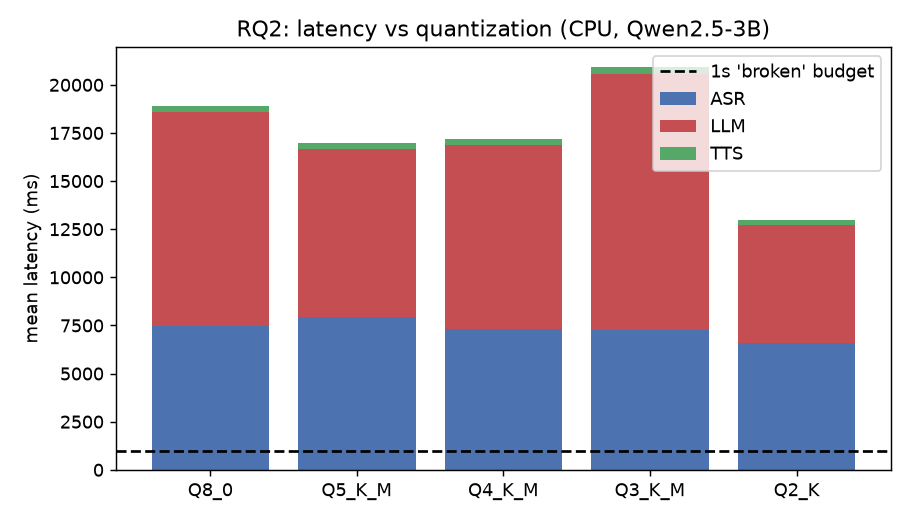
\includegraphics[width=0.72\linewidth]{rq2_quant_sweep.png}
\caption{Stacked per-stage latency by quant level with the 1\,s budget line --- the LLM
dominates and all levels are over budget.}
\label{fig:rq2sweep}
\end{figure}

\begin{figure}[t]
\centering
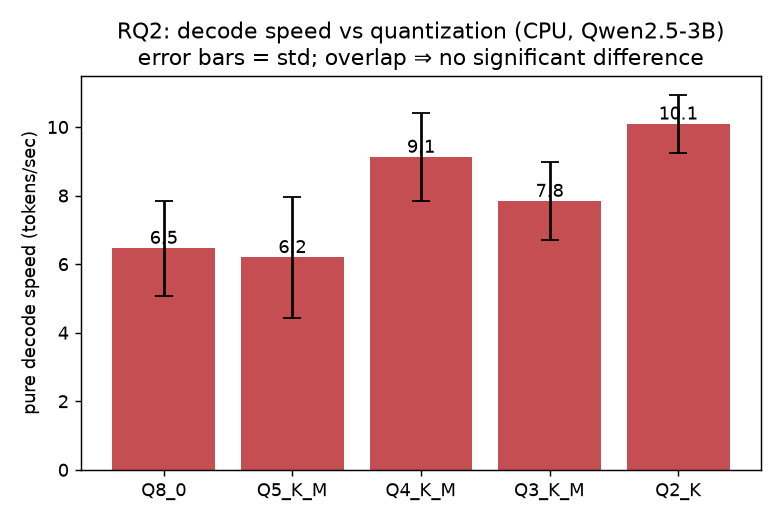
\includegraphics[width=0.62\linewidth]{rq2_quant_speed.png}
\caption{Pure decode speed (tok/s) by quant with $\pm$std error bars ($n{=}20$, two
interleaved trials) --- the ordering is non-monotone and the bands overlap for every
adjacent pair, the visual signature of thermal noise dominating any bit-width effect.}
\label{fig:rq2speed}
\end{figure}

\subsection{RQ1 --- no quantization$\times$noise interaction ($n{=}400$ BFCL, two model
families)}
\label{sec:rq1}
Tables~\ref{tab:qwen} and~\ref{tab:llama} give exact-match under clean and noisy
(synthetic, WER 0.30) input for the extreme quant levels.

\begin{table}[t]
\centering
\begin{minipage}[t]{0.48\linewidth}\centering
\resizebox{\linewidth}{!}{%
\begin{tabular}{lcccc}
\toprule
quant & name (c$\rightarrow$n) & ex.\ clean & ex.\ noisy & $\Delta$ \\
\midrule
Q5\_K\_M & $0.96{\rightarrow}0.96$ & 0.58 & 0.29 & 0.28 \\
Q2\_K    & $0.96{\rightarrow}0.95$ & 0.55 & 0.28 & 0.27 \\
\bottomrule
\end{tabular}}
\caption{Qwen2.5-3B-Instruct.}
\label{tab:qwen}
\end{minipage}\hfill
\begin{minipage}[t]{0.48\linewidth}\centering
\resizebox{\linewidth}{!}{%
\begin{tabular}{lcccc}
\toprule
quant & name (c$\rightarrow$n) & ex.\ clean & ex.\ noisy & $\Delta$ \\
\midrule
Q5\_K\_M & $0.95{\rightarrow}0.95$ & 0.55 & 0.30 & 0.25 \\
Q2\_K    & $0.86{\rightarrow}0.85$ & 0.40 & 0.18 & 0.21 \\
\bottomrule
\end{tabular}}
\caption{Llama-3.2-3B-Instruct.}
\label{tab:llama}
\end{minipage}
\end{table}

\paragraph{No quant$\times$noise interaction, on both models.} The noise penalty
$\Delta$ does not grow for the 2-bit model --- it is equal (Qwen: 0.28 vs 0.27) or
slightly \emph{smaller} (Llama: 0.25 vs 0.21, a floor effect from Llama-Q2's lower
clean baseline). ASR noise roughly halves \code{exact} slot-filling uniformly across
quant levels; \code{valid\_json} stays ${\sim}0.97$ everywhere.

\paragraph{The null replicates under phonetically-grounded noise, on both families.}
The tables above use synthetic word-level corruption; a natural worry is that the null
is an artifact of unrealistic noise, since real ASR errors are acoustic rather than
random. We therefore re-ran both sweeps ($n{=}400$) with a phonetically-motivated noise
model --- voicing confusions (s/z, t/d, k/c), nasal and liquid swaps, reduced-vowel
substitution, and final-consonant drops --- injected to the same 0.30 target WER. The
interaction remains null on both models: \code{exact} $\Delta$(noise) is 0.19
(Q5\_K\_M) vs 0.21 (Q2\_K) for Qwen2.5-3B and 0.16 vs 0.14 for Llama-3.2-3B --- in
neither case does the 2-bit model's noise penalty exceed the 5-bit model's, exactly as
under synthetic noise. Clean baselines reproduce, and Llama's model-specific 2-bit main
effect persists (clean \code{exact} $0.55{\rightarrow}0.40$), so the phonetic model
changes the noise channel without disturbing the standalone quantization cost. Notably
the phonetic model is \emph{gentler} than random-character corruption on both families
(Qwen Q5\_K\_M \code{exact}-under-noise 0.39 vs 0.29; Llama Q5\_K\_M 0.39 vs 0.30) ---
plausibly because acoustic confusions leave more of the target entity recoverable than
character flips do --- so the synthetic figures are, if anything, a conservative upper
bound on noise-induced degradation. Both noise models and both model families agree: no
quant$\times$noise interaction (Fig.~\ref{fig:rq1phon}).

\paragraph{How large an interaction can we exclude?} A null is only as strong as the
effect it can rule out, so we quantify the interaction directly as the contrast
$\Delta(\mathrm{Q2}) - \Delta(\mathrm{Q5})$ --- how much \emph{more} the 2-bit model's
\code{exact} accuracy falls under noise than the 5-bit model's --- with a 95\% CI (each
cell a binomial at $n{=}400$; Table~\ref{tab:ci}). Across all four model $\times$
noise-model combinations the interaction sits within $\pm0.04$ of zero, and every CI
contains zero while excluding any interaction larger than ${\sim}0.13$ exact-match
points. The null is therefore a \emph{bounded equivalence} result --- we can rule out,
at 95\% confidence, any noise$\times$quantization interaction beyond ${\sim}0.1$ ---
not merely a failure to reach significance. The interval is conservative: it treats the
clean and noisy cells as independent, whereas they are paired on the same 400 tasks, so
the true interval is tighter (\code{scripts/interaction\_ci.py} reproduces it).

\begin{table}[t]
\centering
\begin{tabular}{lcccc}
\toprule
model / noise & $\Delta$(Q5) & $\Delta$(Q2) & interaction & 95\% CI \\
\midrule
Qwen2.5-3B / synthetic   & 0.28 & 0.27 & $-0.01$ & $[-0.10, +0.08]$ \\
Qwen2.5-3B / phonetic    & 0.19 & 0.21 & $+0.02$ & $[-0.08, +0.12]$ \\
Llama-3.2-3B / synthetic & 0.25 & 0.21 & $-0.04$ & $[-0.13, +0.05]$ \\
Llama-3.2-3B / phonetic  & 0.16 & 0.14 & $-0.02$ & $[-0.11, +0.07]$ \\
\bottomrule
\end{tabular}
\caption{Interaction contrast $\Delta(\mathrm{Q2})-\Delta(\mathrm{Q5})$ with a
conservative binomial 95\% CI. Every CI contains zero and excludes any interaction
$>{\sim}0.13$.}
\label{tab:ci}
\end{table}

\paragraph{The quantization \emph{main effect} is model-dependent.} Qwen2.5-3B
tolerates 2-bit gracefully (Q2${\approx}$Q5 on clean input). Llama-3.2-3B does not: at
Q2\_K, clean name\_match drops $0.95{\rightarrow}0.86$ ($-9$ pts) and clean exact
$0.55{\rightarrow}0.40$ ($-15$ pts) --- both ${\approx}4\sigma$ at $n{=}400$, i.e.\ real
degradation. So \emph{how much} aggressive quantization costs on clean input depends on
the model family, but \emph{whether noise compounds it} does not --- the interaction is
null for both.

\begin{figure}[t]
\centering
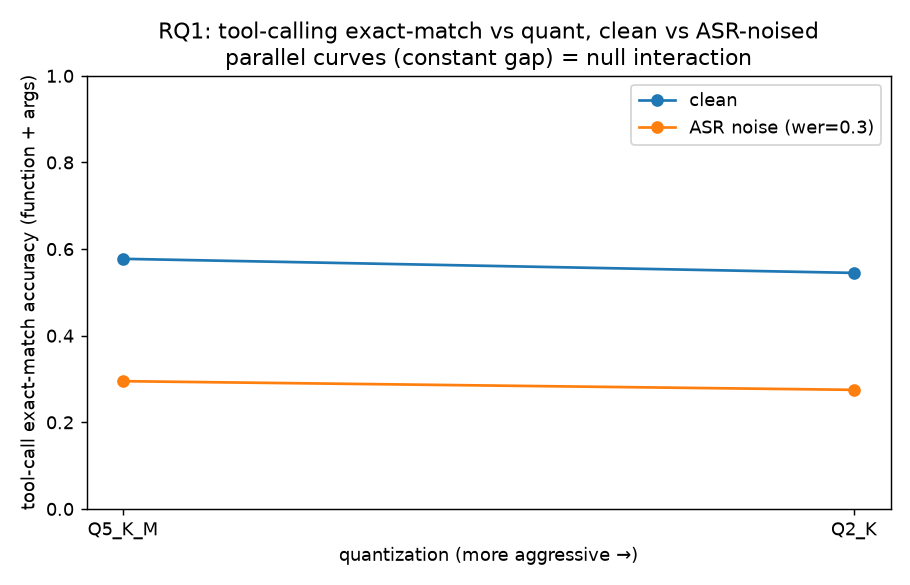
\includegraphics[width=0.62\linewidth]{rq1_interaction.png}
\caption{Tool-call \code{exact}-match accuracy vs quant level, clean vs ASR-noised
(Qwen2.5-3B, synthetic noise, $n{=}400$) --- the clean and noisy curves stay parallel
(constant ${\sim}0.28$ gap) rather than diverging at low bits, the visual signature of
a null interaction.}
\label{fig:rq1syn}
\end{figure}

\begin{figure}[t]
\centering
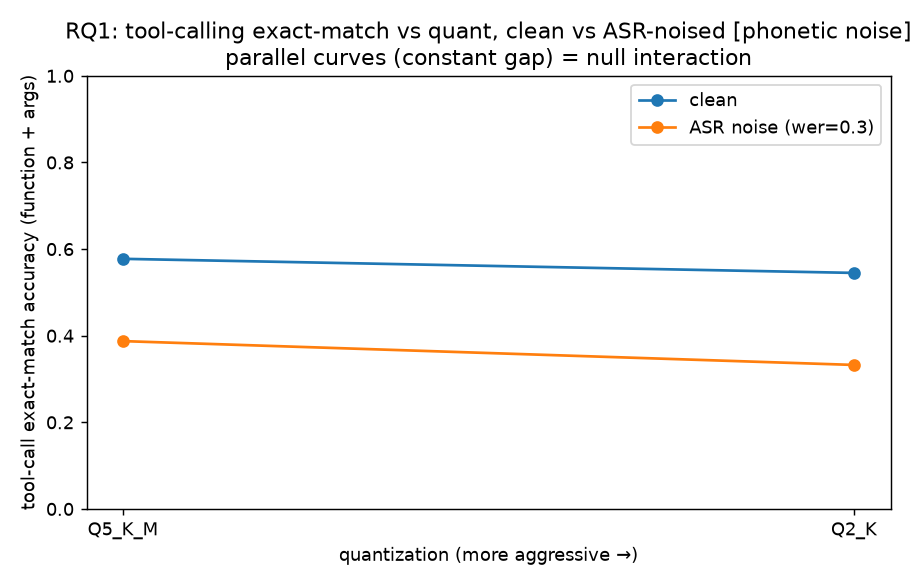
\includegraphics[width=0.62\linewidth]{rq1_interaction_phonetic.png}
\caption{The same sweep under phonetically-grounded noise --- identical parallel
structure, confirming the null is not an artifact of the synthetic noise model.}
\label{fig:rq1phon}
\end{figure}

\paragraph{A cautionary intermediate result.} An earlier 4-quant Qwen sweep at
$n{=}80$ produced an apparently \emph{monotonic} interaction --- exact $\Delta$(noise)
of 0.21, 0.26, 0.29, 0.31 for Q5/Q4/Q3/Q2 --- that looked like clear support for the
low-bit-fragility hypothesis. Decomposition showed it was an artifact: the noisy values
had converged (Q5 and Q2 both ${\approx}0.34$), and Q2's larger $\Delta$ rode entirely
on an implausibly high \emph{clean} baseline (Q2 clean exact $0.65 > {}$Q5's 0.55) ---
sampling noise at $n{=}80$. Scaling to $n{=}400$ erased the effect. We report this
because it illustrates a methodological point (\S\ref{sec:disc}): interaction effects
must be decomposed into their clean and noisy components and powered adequately, or
proportion noise at small $n$ masquerades as a trend.

\section{Discussion}
\label{sec:disc}
\begin{itemize}
\item \textbf{Quantization is cheap for tool-calling quality, an unreliable lever for
CPU latency.} The two deployment levers point opposite ways from intuition.
\item \textbf{ASR noise, not weight precision, is the quality bottleneck} --- and it
hits argument slot-filling specifically (entity recovery), not function selection.
Implication: invest in ASR quality / noise-robust slot extraction, not higher
bit-width.
\item \textbf{The interaction null generalizes; the main effect does not.} Across two
model families the \emph{absence} of a quant$\times$noise interaction is consistent, but
the standalone clean-input cost of 2-bit differs sharply (Qwen2.5-3B robust;
Llama-3.2-3B loses ${\sim}15$ pts exact). Llama's loss includes a 9-pt drop in
function selection (\code{name\_match} $0.95\rightarrow0.86$), in line with the
tool-name hallucination \citet{jang2026} find quantization amplifies on
$\tau^2$-bench; Qwen shows no such drop, so that effect too is model-dependent.
The two results are complementary: quantization can amplify a model's existing
tool-calling failures, but ASR noise does not amplify them further. Practitioners
should pick a quant level by
testing their specific model on clean input --- and can then trust that ASR noise won't
disproportionately amplify that choice.
\item \textbf{Methodological:} decode-latency benchmarks of quantized LLMs on laptops
must control thermal throttling; quality metrics must use greedy decoding and decompose
$\Delta$ into clean/noisy components (an apparent $n{=}80$ interaction vanished at
$n{=}400$); and a claimed null interaction should be reported as a CI / equivalence
bound (what effect size can we \emph{exclude}?), not just a non-significant point
estimate.
\end{itemize}

\section{Limitations}
Two model families (Qwen2.5-3B, Llama-3.2-3B), both ${\sim}3$B --- larger/smaller scales
untested; single CPU; word-level noise --- both a synthetic and a phonetically-grounded
model (the interaction null holds under both), but not real round-trip
TTS$\rightarrow$ASR errors, whose WER is pipeline-determined and which remain the one
untested noise source; BFCL \code{simple} (single-turn, small per-task catalogs make
\code{name\_match} saturate; multi-turn BFCL v3 untested); latency numbers from a
thermally-variable laptop (structure reproduces; absolute ms will not). The interaction
null is shown for tool-calling; other capabilities (multi-turn dialogue coherence,
long-context) are not covered.

\section{Conclusion}
On-device voice agents can be quantized aggressively (to 2-bit) with negligible
tool-calling cost, clean or noisy; quantization and ASR noise degrade quality through
independent channels, not a compounding cliff. The binding constraints are latency
(LLM-dominated, over budget, not reliably reduced by quantization on CPU) and ASR
quality (the true driver of slot-filling errors).

\begin{thebibliography}{99}
\small
\bibitem[Dong et al.(2025)]{dong2025} Dong, P., Tang, Z., Liu, X., Li, L., Chu, X.,
\& Li, B. (2025). \emph{Can Compressed LLMs Truly Act? An Empirical Evaluation of
Agentic Capabilities in LLM Compression} (ACBench). ICML 2025. arXiv:2505.19433.
\bibitem[Dutta et al.(2024)]{dutta2024} Dutta, A., Krishnan, S., Kwatra, N., \&
Ramjee, R. (2024). \emph{Accuracy is Not All You Need.} NeurIPS 2024. arXiv:2407.09141.
\bibitem[Ethiraj et al.(2025)]{ethiraj2025} Ethiraj, V., David, A., Menon, S., \&
Vijay, D. (2025). \emph{Toward Low-Latency End-to-End Voice Agents for
Telecommunications Using Streaming ASR, Quantized LLMs, and Real-Time TTS.}
arXiv:2508.04721.
\bibitem[Fang et al.(2025)]{fang2025} Fang, S., Ding, W., Mastropaolo, A., \& Xu, B.
(2025). \emph{Smaller = Weaker? Benchmarking Robustness of Quantized LLMs in Code
Generation.} arXiv:2506.22776.
\bibitem[Huang et al.(2025)]{huang2025} Huang, S., et al. (2025). \emph{AdaSpec:
Adaptive Speculative Decoding for Fast, SLO-Aware LLM Serving.} ACM SoCC 2025.
arXiv:2503.05096.
\bibitem[Jang et al.(2026)]{jang2026} Jang, J., Yang, K., Lim, H., \& Park, H. (2026).
\emph{Flat Score, Amplified Failures: How the Error Budget Masks Damage in Quantized
LLM Agents.} arXiv:2607.27275.
\bibitem[Kurt(2026)]{kurt2026} Kurt, U. (2026). \emph{Which Quantization Should I Use?
A Unified Evaluation of llama.cpp Quantization on Llama-3.1-8B-Instruct.}
arXiv:2601.14277.
\bibitem[Laskar et al.(2026)]{laskar2026} Laskar, M. T. R., Fu, X.-Y., Sarfjoo, S. S.,
McNamara, Q., Robertson, J., \& TN, S. B. (2026). \emph{From Text to Voice: A
Reproducible and Verifiable Framework for Evaluating Tool Calling LLM Agents.}
arXiv:2605.15104.
\bibitem[Lee et al.(2024)]{lee2024} Lee, J., et al. (2024). \emph{A Comprehensive
Evaluation of Quantized Instruction-Tuned LLMs: An Experimental Analysis up to 405B.}
arXiv:2409.11055.
\bibitem[Li \& Grover(2025)]{li2025predgen} Li, S., \& Grover, A. (2025).
\emph{PredGen: Accelerated Inference of LLMs through Input-Time Speculation for
Real-Time Speech Interaction.} COLM 2025. arXiv:2506.15556.
\bibitem[Li et al.(2024)]{li2024} Li, S., et al. (2024). \emph{Evaluating Quantized
Large Language Models.} ICML 2024. arXiv:2402.18158.
\bibitem[Likhomanenko et al.(2025)]{likhomanenko2025} Likhomanenko, T., et al. (2025).
\emph{ChipChat: Low-Latency Cascaded Conversational Agent in MLX.} arXiv:2509.00078.
\bibitem[Lv et al.(2025)]{lv2025} Lv, K., et al. (2025). \emph{DuoDecoding:
Hardware-aware Heterogeneous Speculative Decoding with Dynamic Multi-Sequence
Drafting.} arXiv:2503.00784.
\bibitem[Patil et al.(2024)]{patil2024} Patil, S. G., et al. (2024). \emph{Berkeley
Function-Calling Leaderboard (BFCL).} \url{https://gorilla.cs.berkeley.edu}.
\bibitem[Peng et al.(2026)]{peng2026} Peng, Y., Liu, Y., Gao, C., Gao, Z., Chen, Q.,
Li, X., \& Chen, X. (2026). \emph{Spoken Function Calling: A New Perspective on Spoken
Language Understanding for Large Audio Language Models.} arXiv:2608.05126.
\bibitem[Song et al.(2025)]{song2025} Song, Q., et al. (2025). \emph{A Systematic
Evaluation of On-Device LLMs: Quantization, Performance, and Resources.}
arXiv:2505.15030.
\bibitem[Stivers et al.(2009)]{stivers2009} Stivers, T., et al. (2009). \emph{Universals
and cultural variation in turn-taking in conversation.} PNAS 106(26):10587--10592.
\bibitem[Wang et al.(2026)]{wang2026} Wang, R., et al. (2026). \emph{AgentNoiseBench:
Benchmarking Robustness of Tool-Using LLM Agents Under Noisy Condition.}
arXiv:2602.11348.
\end{thebibliography}

\end{document}
